\documentclass[11pt]{article}

\usepackage{epsfig}
\usepackage[pdftex,bookmarks=true,bookmarksnumbered=true,colorlinks]{hyperref}
\usepackage{xspace}
\usepackage{a4wide}
%\usepackage{typearea}
%\areaset[1cm]%               % Zusaetzlicher Rand fuer die Bindung
%{15cm}{20cm} 

\newcommand{\key}[1]{\texttt{[#1]}}
\newcommand{\userinput}[1]{\texttt{#1}}
\newcommand{\term}[1]{\textsf{#1}}
\newcommand{\useroption}[1]{\textsf{#1}}
\newcommand{\operator}[1]{\textsf{#1}}
\newcommand{\parameter}[1]{\textsf{#1}}

\newcommand{\rapidminer}{\protect \textsc{RapidMiner}\xspace}

\title{The \rapidminer GUI Manual}


\begin{document}

\maketitle


\abstract{This document describes the usage of the graphical user
interface (GUI) of the data mining software package \rapidminer. Since the
interface was intended to ease the usage of \rapidminer avoiding handling of XML
configuration files, there should be almost nothing to
explain. Hence this document describes the very basic ideas of \rapidminer and their
representations in the GUI. We suggest that you first make the online tutorial 
and read this document. After that, you will find it much easier to read the \rapidminer 
Tutorial and skip a lot of its contents.}

\tableofcontents


\section{General Information}

Although the \rapidminer tutorial and this GUI manual contain a huge amount
of information about \rapidminer and all of its parts, it is often very
convenient to get the desired information during work. Therefore, we 
added an online help function to almost all parts of \rapidminer. Each
parameter, operator and GUI item displays information as tool tip text,
which appears after holding the mouse cursor a few moments above the
object at hand.

\section{Setting up a Process}

When \rapidminer starts up, it presents you a welcome screen that lets
you choose between five possibilities
\begin{itemize}
\item Start with a blank process setup
\item Open one of the recently used process definitions
\item Open an existing process definition
\item Start the Process Creation Wizard
\item Start the \rapidminer online tutorial
\end{itemize}

\subsection{The online tutorial}

When you start \rapidminer the first time, you should probably make the online
tutorial. It explains the main concepts, the GUI usage and shows
many of the operators provided by \rapidminer.

\subsection{The Wizard}

We assume that you have chosen to start the Wizard (figure
\ref{fig:wizard_template}). The Wizard is also available from the
\useroption{File} menu. The Wizard guides you during the process of
creating a new process. You start by selecting a template
process from a list. This template serves as a kind of skeleton for
your process.
\begin{figure}[ht]
\center
\includegraphics[width=0.88\linewidth]{screenshot_template_valid.png}
\caption{The \rapidminer Process Creation Wizard is a simple way to create basic process definitions.}
\label{fig:wizard_template}
\end{figure}

Processes in \rapidminer are made up from a set of nested operators. An
operator consumes a set of input objects and produces some output
objects. These objects can be data files, models, performance criteria,
and more. Simple operators like learners consume an example set and
produce a model that can be used by an applier for
prediction. Moreover, some operators can have inner operators. For example, a
$k$-fold cross-validation splits up an example set into training set
and test set and applies its inner operators, which are a learner and
an applier. Each time a disjoint test set is used.


If you click on the radio button next to the "SVM with XValidation"
template, the structure of the sample process is depicted on the
right. You see an operator chain consisting of an
\operator{ExampleSource} that reads data from a file. This data is
then passed to the cross-validation, which itself has inner operators,
in this case learner and applier for a support vector machine
(SVM). See the \rapidminer Tutorial for more information on SVMs and the
individual operators.

Now that you have chosen the template, click on \useroption{next}. In
this step you can enter some of the most important parameters (figure
\ref{fig:wizard_parameter_editing}). In case of a cross-validation
this is e.\,g. the number of validations.
\begin{figure}[ht]
\center
\includegraphics[width=0.88\linewidth]{screenshot_template_edit_parameter.png}
\caption{The parameter editing step of the Wizard.}
\label{fig:wizard_parameter_editing}
\end{figure}

A lot of process setups in \rapidminer need a data file as input which is known in supervised 
learning as an example set. The example sets have to be in a special format and require
that the attributes are described in a seperate XML file. In other words, the file in special 
format is the set of examples where each example is a vector and the XML file describes the 
semantics of every value in the vector. 

In order to create such an XML file now, you can press the small
\userinput{Edit} button next to an attribute description file
property. The dialog popping up is described in section
\ref{sec:attribute_editor} and is called Attribute Editor. The files
generated with help of the Attribute Editor can also be used as input
for the ExampleSource operator, which is the standard data input
operator for \rapidminer.

\subsection{Operator Configuration Wizards}

An even more convenient way of loading almost arbitrary data files into \rapidminer 
and to define attribute description files for your data, is to use the Example 
Source configuration wizard. Just press the \emph{Start Configuration Wizard\ldots} 
button at the top of the parameter table of the operator. Configuration wizards are 
also available for other operators which are hard to define, e.g. for the DatabaseExampleSource
operator.




\subsection{The tree view and other process views}

As operators can have inner operators and each operator except the
root operator is enclosed within another operator, the natural
representation of an process is a tree. If you have used the
Wizard, you see your process definition on the left side. If you did not use the Wizard
you see an empty process consisting only of an empty operator
chain. Figure \ref{fig:main_experiment_view} shows this main
process view which is called ``tree view''.
\begin{figure}[ht]
\center
\includegraphics[width=0.88\linewidth]{main_experiment_view.png}
\caption{Main tree view of the process editor window.}
\label{fig:main_experiment_view}
\end{figure}

By clicking on the \useroption{XML} tab you see the XML configuration
file that describes your process (figure
\ref{fig:wizard_xml_editing}). If you like you can always edit it by
hand using your favorite text editor. For more information about the
XML configuration files see the \rapidminer Tutorial.
You can specify HTML comments to each operator in the \useroption{Comment} tab which are
saved in the XML files. If you specify a comment for the root operator
of the process, this comment is displayed in a dialog each time the
process setup was loaded.
Selecting the 
\useroption{Box View} from the View menu shows a nicer box representation of your
process you already know from the Wizard. You can use this view for
printing.
\begin{figure}[ht]
\center
\includegraphics[width=0.88\linewidth]{screenshot_xml_edit.png}
\caption{The \rapidminer XML configuration editor }
\label{fig:wizard_xml_editing}
\end{figure}






\subsubsection{Editing parameters}

To the right of the tree you see a table with two columns labeled ``Key''
and ``Value''. Depending on the selected operator you can enter the
parameters of this operator. Mandatory parameters are shown in bold
face. Some of the parameters may have a default value, which will be
used if no other value was specified. If the entered value
is out of range, it will be corrected automatically. Some
parameters accept only numbers, others let you select from a list of
values. For file parameters, the file name can be entered into the text
field or the file is selected by means of a file chooser dialog, that
pops up when pressing the \useroption{[...]} button. All file names
can be defined relatively against the location of the process definition
file. Of course this only works after the process was saved.

\paragraph{Tip:} Keep the mouse cursor a few moments above a
parameter. Useful information about the parameter will be displayed
as tool tip text.



\subsection{Creating, deleting, moving and replacing operators}

If you started with a blank process setup or you want to modify an
process created by the Wizard, the thing you probably want to do is
create a new operator. 

Since this feature seemed most important to us
it is accessible from many places: from the \useroption{Edit} menu,
the icon bar below the menu bar, the "New Operator" tab, the context
menu popping up whenever you right-click on an operator of the tree,
or simply by pressing \key{Ctrl-I}. Figure \ref{fig:operator_new}
shows the icon for operator adding.
\begin{figure}[ht]
\center
\includegraphics[width=0.08\linewidth]{new_operator.png}
\caption{The new operator icon.}
\label{fig:operator_new}
\end{figure}

Whichever way you choose to activate this function, it
will pop up an operator browser that lets you choose the operator type
(select a group or input or output types first if you want to decrease
the number of possible selections). This browser displays all
available information about the currently selected operator. You
should name the operator before you add it into your
process. You can always rename an operator by pressing \key{F2} or
triple clicking it in the tree view. Figure
\ref{fig:operator_selection} shows the operator browser. 
\begin{figure}[ht]
\center
\includegraphics[width=0.88\linewidth]{operator_selection.png}
\caption{The Operator Browser for information and operator adding.}
\label{fig:operator_selection}
\end{figure}

Another way to add an operator is to right click on the parent
operator and select the operator from the \useroption{New operator}
submenu. Adding operators directly from the context menu is a very
fast way of process design. Both ways of adding are only possible
if an operator chain is selected, i.e. an operator which can have
children.

\paragraph{Tip:} Keep the mouse cursor a few moments above an
operator in the submenus. Useful information about the operator will
be appear as tool tip text.

\medskip

You can replace an operator by selecting the new operator from the
submenu \useroption{Replace operator} of the context menu. This is
similar to adding a new operator from the context menu instead of
using the operator browser. When you replace an operator chain 
the inner operators will remain. Therefore, operator chains containing
any children can only be replaced by other operator chains.

\medskip


Removing the operator is even easier. Just press
\key{Delete} or select the corresponding menu item from the context
menu or the \useroption{Edit} menu. Figure \ref{fig:operator_delete}
shows the icon for operator deleting.
\begin{figure}[ht]
\center
\includegraphics[width=0.08\linewidth]{delete_operator.png}
\caption{The remove operator icon.}
\label{fig:operator_delete}
\end{figure}

You can use the ``Drag \& Drop'' functionality
to move an operator up or down within the tree.






\subsection{Operator info}

Pressing \key{F1} brings up a dialog with useful information about
the currently selected operator. This option is also available from
the context menu of each operator or the \useroption{Tools} menu. This
operator info dialog displays:
\begin{itemize}
\item a short description
\item which input the operator demands
\item which output the operator delivers
\item the minimum number of inner operators, if the selected operator
  can have children
\item the maximum number of inner operators, if the selected operator
  can have children
\item errors in process setup (if errors exist)
\item a description or comment text field
\end{itemize}





\subsection{The attribute editor}
\label{sec:attribute_editor}

Example sets or instance sets in \rapidminer are described by using a separate XML
document. This attribute description file contains information about
the type of data and its source. Data sets can be distributed over
several files. This may be particularly useful if the label is stored
within a file of its own. The \rapidminer Tutorial will give help in case you
want to edit this file yourself.


The GUI displays a small \useroption{Edit} button next to an attribute
description file property (e.\,g. the parameter \parameter{attributes} of an
\operator{ExampleSource}) in the property editor. A dialog called
Attribute Editor will pop up containing a table with one column for
each attribute (figure \ref{fig:attribute_editor}). If the property
does not yet reference a proper attribute description file, the dialog
will be empty. If you want to follow the instructions below, which describe 
how to create the XML description file, you can clear the table by clicking on
the corresponding button above the table, or selecting "Clear" from the "Table" menu, 
to start from scratch.
\begin{figure}[ht]
\center
\includegraphics[width=0.08\linewidth]{clear_button.png}
\caption{The clear button.}
\label{fig:attribute_editor}
\end{figure}

\begin{figure}[ht]
\center
\includegraphics[width=0.88\linewidth]{attribute_editor.png}
\caption{The Attribute Editor dialog for data loading and attribute
  description file creation.}
\label{fig:attribute_editor}
\end{figure}


Assume, you have a data file containing 50 rows of whitespace or comma
separated attribute values, five each  row. Click on load data to open
that file. After that you should see five columns with some headers each
and the data in the table cells. Question marks (``?'') indicate missing
values. The following enumeration explains the meanings of the table headers:
\begin{enumerate}
\item The first header row contains the source file and column index. This
  is not editable but just for your information.
\item The second row shows the name of each column. You can edit the name by
  clicking into the text field.
\item The third row indicates, what the data is used for. For example, it can
  be an ordinary attribute, a label for classification or
  regression tasks, or a weight that can be used with certain
  algorithms. There can be at most one label and one weight attribute.
\item The fourth row is the value type. Most interesting are
  the choices \term{real} / \term{integer} and \term{nominal}. \rapidminer
  should have automatically detected these correctly.
\item The last header row is the block type. Most interesting are
  \term{single\_value} (default) and \term{value\_series}. For some
  processes, value series are treated in a special way. Do not forget
  to assign \term{value\_series\_\-start} and \term{value\_series\_end} to
  the first and last column respectively.
\end{enumerate}
You can change the values according to your needs and load an
arbitrary number of data files. Finally click on \useroption{Save
attribute description file}, which you can find in the file menu,
to write the XML file to disk, or just click on the "Save" button.
\begin{figure}[ht]
\center
\includegraphics[width=0.08\linewidth]{save_button.png}
\caption{The button for saving an attribute description file.}
\label{fig:operator_delete}
\end{figure}

\paragraph{Tip:}
If you do not want to use this \rapidminer standard data format, you can use
one of the provided special format operators which can read Arff
files, comma separated value files (csv), bibtex files, dBase files,
C4.5 files, and more.

\paragraph{Tip:}
An even more convenient way of loading almost arbitrary data files into \rapidminer 
and to define attribute description files for your data is to use the Example 
Source configuration wizard. Just press the \emph{Start Configuration Wizard\ldots} 
button at the top of the parameter table of the operator. Configuration wizards are 
also available for other operators which are hard to define, e.g. for the DatabaseExampleSource
operator. The wizards are self explaining, just follow the steps and read the instructions.



\section{Validating your process definition}

Before you run your process you should validate it.
You can click on
\useroption{Validate Process} in order
to check if all operators are nested correctly, provided with their
necessary input and 
mandatory properties are set (figure
\ref{fig:validate_experiment_button}). Although this might be useful,
you do not need to do it manually, since these checks are performed
automatically before the process is started. 
\begin{figure}[ht]
\center
\includegraphics[width=0.08\linewidth]{validate_button.png}
\caption{The validate process icon.}
\label{fig:validate_experiment_button}
\end{figure}

The result of the validation including all error messages is printed into the 
message viewer at the bottom of the main frame.
Additionally, they are indicated by an
exclamation mark next to the operator in the tree view. An example is
shown in figure \ref{fig:error_message}. You can display these
messages and more information about the operator by 
pressing \key{F1} or selecting the \useroption{Operator info} menu item
from the context menu or from the \useroption{Tools} menu.
\begin{figure}[ht]
\center
\includegraphics[width=0.88\linewidth]{error_message.png}
\caption{Error Messages in the Message Viewer (lower part)
  highlighting the errors in the process.}
\label{fig:error_message}
\end{figure}


Process validation is very important in order to create proper process definitions
and can help to understand the concepts of \rapidminer. We therefore recommend to use
process validation as often as possible, at least once before you start
your process. Together with the breakpoints from the operator context menu,
it is usually much easier to design new or complex processes.



\section{Running your process}

Running your process is quite easy. Select \useroption{Run}
from the \useroption{Process} menu or click the corresponding
play button, which is shown in figure \ref{fig:play_button}.
\begin{figure}[ht]
\center
\includegraphics[width=0.08\linewidth]{play_button.png}
\caption{The process run icon.}
\label{fig:play_button}
\end{figure}

You may follow the progress of your process by observing the output
which is displayed in the Message Viewer. Note, that in GUI mode, the
output does not need to be written to a log file. If you did not
specify a log file, you can always save the message viewer contents to
a file by selecting the corresponding menu item in the Message
Viewer's context menu. You can also perform a search in the Message
Viewer. This option is also accessible from the context menu of the
viewer.

\paragraph{Tip:}
The amount of logging messages can be defined by the parameter
\useroption{log\_verbosity} of the Process operator (the root of the
process tree). This operator also provides other parameters useful
for the complete process.





\section{Evaluating the results}

When your process is finished, the results will be automatically presented,
i.\,e. all output returned by the outermost operator. This can
be performance statistics, a decision tree or anything else. \rapidminer
automatically selects the \useroption{Results Mode}.
You can switch between the \useroption{Edit Mode} and the \useroption{Results Mode}
by clicking on the two buttons in the top right corner, or by selecting the mode
in the View menu. Pressing the hotkey \key{F9} is another possibility to toggle
between both modes.

When your process was conducted successfully, the view
automatically switches to the \useroption{Results Mode}. As far as your
process chain produces an output, this mode shows you a
visualization or a text describing the output. Figure
\ref{fig:screenshot_tree} shows a decision tree learned from the golf
data set.
\begin{figure}[ht]
\center
\includegraphics[width=0.88\linewidth]{decision_tree.png}
\caption{A decision tree as result of a learning process.}
\label{fig:screenshot_tree}
\end{figure}

At any time you can stop or pause (and resume) the process using
the appropriate buttons or menu items in the \useroption{Process}
menu. In any case the operator currently being executed will finish
its execution in the background. Since this might take some time (e.g. if the current
operator was a learner) this might lead to a delay for the actual process
termination. Please be patient. You can, however, directly start and perform changes to
the current process setup and even restart the process.

If you want to observe your process closely, you can set
breakpoints before and after every operator (via the operator context
menu). In that case, each time a breakpoint is reached, intermediate
results are presented similar to the dialog popping up at the end of
the process.
You can see a plot of the memory usage and the progress bar.




\subsection{Plotter}

In case you used the \operator{ProcessLog} operator, you
also find the produced plots as shown in figure
\ref{fig:screenshot_plot}. The results can be viewed online during the
run of a process. On the left hand side you can select the
value that is assigned to the x-axis and one or more of the values
that should be plotted on the y-axis. The example shows a plot of the
absolute error depending on the SVM parameter $C$ and $degree$. 

Additionally, the standard scatter plotter can use three dimensions. There are two 3D
plot modes integrated in \rapidminer. The first one (3D (color) scatter plot)
produces 3D plots, which can be rotated by dragging the 
mouse over the plot. The second 3D plot mode of \rapidminer is the 2D
color plot mode. The first two dimensions build an 2D layer and the
third dimension is mapped on different colors or alternatively different
sizes. Other plotters exist
for scatter plots or histograms. Table \ref{tab:plotters_overview} gives an
overview over all existing plotters.

There exist several objects which can also be plotted, e.g. Example sets
have a meta data view, a data view, and a plot view. In plot view some
features can be selected to build the dimensions of a plot. Figure
\ref{fig:plot_iris} gives an example for the plot view of the well
known Iris dataset.


\begin{table}[htbp]
  \begin{tabular}{|l|l|}
    \hline
    \textbf{Plotter} & \textbf{Description} \\
    \hline
    Scatter           & A 2D scatter plot which is also capable of plotting lines \\
                      & and a third dimension by colorizing the third dimension \\
    Scatter Matrix    & A matrix plot of scatter plotters \\
    Scatter 3D        & A 3D scatter plot \\
    Scatter 3D Color  & A 3D scatter plot colorizing a 4th dimension \\
    Bubble            & A 2D plot using the size of each bubble to represent \\
                      & a third dimension \\
    Parallel          & Each dimension is plotted on parallel coordinates \\
    Survey            & A survey plot plotting sorted histograms in parallel \\
    SOM               & A Self-Organizing Map plot using a Kohonen net for \\
                      &  dimensionality reduction \\
    Density           & A 2D plotter using two dimensions as axis, one dimension \\
                      &  as density color, and one dimension for point colors \\
    Pie               & A 2D pie chart (allows group by aggregation average) \\
    Pie 3D            & A 3D pie chart, like 2D but with depth and transparency \\
    Ring              & A ring plot, like the 2D pie chart \\
    Andrews Curves    & Parallel coordinates after a sort of Fourier transform \\
    Histrogram        & A histogram plot for one of the dimensions \\
    Histrogram Color  & A histogram plot for one of the dimensions where the \\
                      & values are binned according to another dimension \\
    Histrogram Matrix & A histogram plot for all dimensions \\
    Histrogram Color Matrix & A color histogram plot for all dimensions binned \\
                            & by one (nominal) dimension beforehand \\
    Quartile          & A quartile plot (aka box plot) for one of the dimensions \\
    Quartile Color    & A quartile plot for one of the dimensions where the \\
                      & values are binned according to another dimension \\
    Quartile Color Matrix   & A color quartile plot for all dimensions binned \\
                            & by one (nominal) dimension beforehand \\
    Sticks            & A stick plot, similar to the bars plot \\
    Sticks 3D         & A 3D stick plot \\
    Bars              & A 2D bar chart (allows group by aggregation average) \\
    Bars 3D           & A 3D bar chart, like 2D but with depth \\
    Box               & A 2D scatter plot where another dimension can define a \\
                      & box around the points (often used for variance) \\
    Box 3D            & A 3D scatter plot where another dimension can define a \\
                      & box around the points (often used for variance) \\ 
    RadViz            & A plotter with radial visualisation anchors \\
    GridViz           & A plotter with grid visualisation anchors \\
    Surface 3D        & A 3D surface plot (only available for less data points) \\
    \hline
  \end{tabular}
  \caption{A collection of all \rapidminer plotters.}
  \label{tab:plotters_overview}
\end{table}



\subsubsection{Zooming}

Drag a rectangle to zoom into the selected range. Right click sets the
view back to maximal range. This type of zooming is only supported for the 2D
scatter plots. For some of the other plotters zooming might be implemented
during a slider in the options pane on the left or even by simply turning the
mouse wheel.


\begin{figure}[htbp]
\center
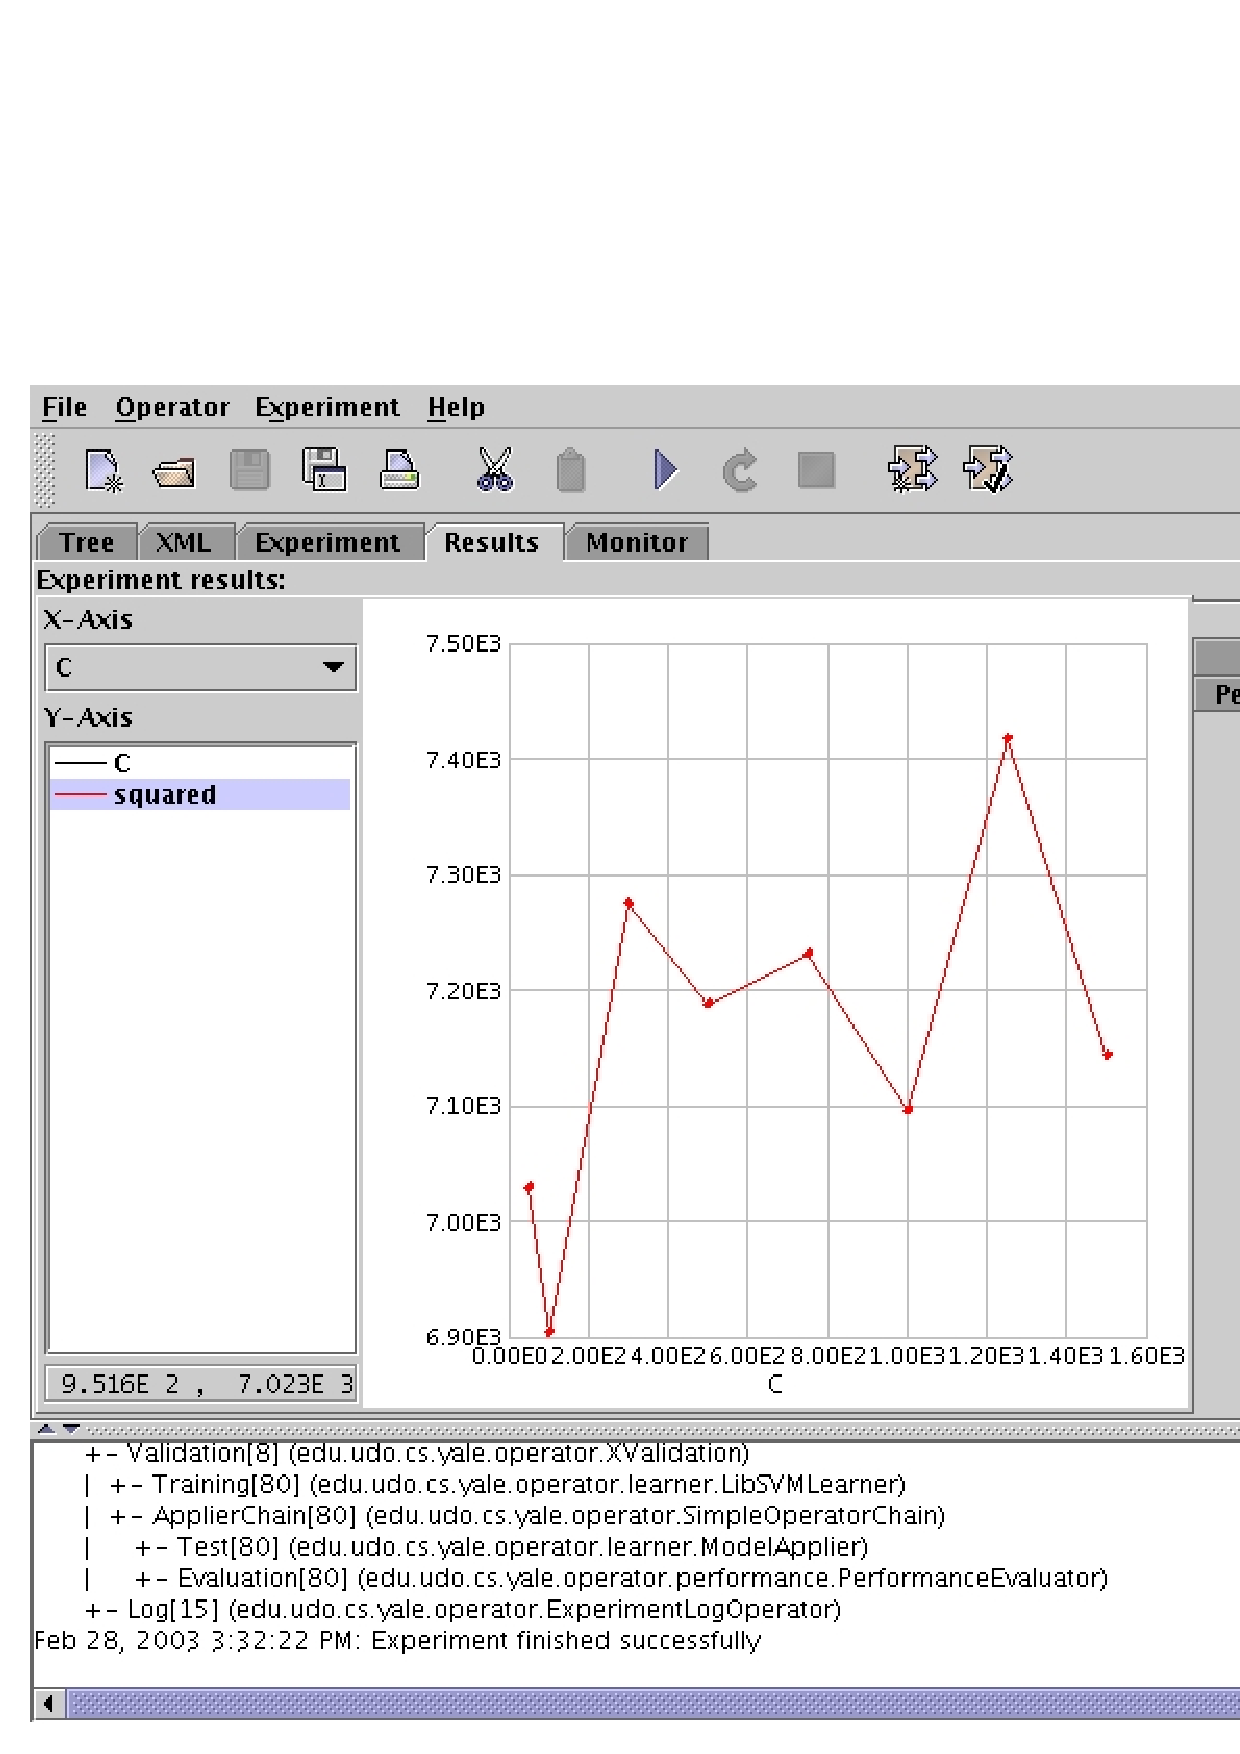
\includegraphics[width=0.88\linewidth]{screenshot_plot.png}
\caption{A plot of a parameter optimization run.}
\label{fig:screenshot_plot}
\end{figure}


\begin{figure}[htbp]
\center
\includegraphics[width=0.88\linewidth]{plot_iris.png}
\caption{A plot of the well known Iris example set}
\label{fig:plot_iris}
\end{figure}




\section{Settings}

You can open a dialog for global settings (Preferences) from the \useroption{Tools}
menu.
These settings specify the behavior of \rapidminer for different tasks, 
e.g. if the system should beep at the end of an process or how many 
examples (data points) are displayed in the result viewer. The settings 
dialog allows to set all global properties described in the \rapidminer 
tutorial, including the path to the executables of external programs. 
You can apply the changed settings only for the current session or 
save them for future sessions.


\end{document}